%% Normalidade Contextual em APIs -- versão reescrita (apoio à triagem de incidentes)
%% Classe acmart (sigconf), compatível com Overleaf (pdfLaTeX, XeLaTeX ou LuaLaTeX).
\documentclass[sigconf,nonacm]{acmart}

\usepackage[brazilian]{babel}
\usepackage{booktabs}
\usepackage{multirow}
\usepackage{amsmath}
\usepackage{xspace}
\usepackage{fancyvrb}

\citestyle{acmauthoryear}
\settopmatter{printacmref=false, printfolios=true}
\renewcommand{\keywordsname}{Palavras-chave}

\setlength{\emergencystretch}{1.5em}

\newcommand{\Normal}{\textsc{Normal}\xspace}
\newcommand{\Residual}{\textsc{Residual}\xspace}

\begin{document}

\title{Normalidade Contextual em APIs: Caracterização de Regimes a partir de Access Logs para Apoio à Triagem de Incidentes}

\author{Diego Paz Casagrande}
\affiliation{%
  \institution{Universidade de Brasília}
  \city{Brasília}
  \state{DF}
  \country{Brasil}}

\renewcommand{\shortauthors}{D. P. Casagrande}

\begin{abstract}
Na triagem de um incidente, o operador precisa saber se as APIs envolvidas estavam operando normalmente antes do registro e, se não estavam, como, desde quando e de que lado da integração está o desvio. Essa resposta não é trivial porque o comportamento de uma API não é estacionário: volume, latência e taxa de erro variam legitimamente com o horário, o calendário e os processamentos em lote. Este trabalho investiga se atributos estatísticos derivados exclusivamente de \emph{API Access Logs} (AALs) agregados permitem caracterizar os múltiplos comportamentos normais de cada recurso de API e classificar períodos como \Normal ou \Residual, gerando uma informação explicável para apoiar a triagem. Seguindo o CRISP-DM, propõe-se um perfil de normalidade contextual por recurso (mediana e MAD por hora e tipo de dia), com limite próprio para cada atributo e limiar calibrado por validação cruzada, e uma matriz heurística que indica o lado provável da falha (provedor ou consumidor). Em 2,3 milhões de registros de 12 recursos de uma instituição financeira, os testes estatísticos confirmaram regimes ligados à hora do dia em todos os recursos. Na avaliação com 440 episódios de falhas injetadas, o método obteve F1 por episódio de 0,41, contra 0,33 a 0,38 dos baselines, com 0,6\% de alarmes em janelas limpas. Nas consultas pré-incidente, o início do desvio foi estimado com erro mediano de até 0,1~h e o lado provável acertou 92,8\% dos episódios detectados. A sensibilidade, porém, é limitada: 30\% dos episódios, com baixa detecção de desvios de volume.
\end{abstract}

\keywords{Mineração de Dados; API Access Log; Normalidade Contextual; Triagem de Incidentes; CRISP-DM; Regimes Operacionais.}

\maketitle

%% =====================================================================
\section{Introdução}

A arquitetura dos sistemas modernos consolidou o uso de APIs (\emph{Application Programming Interfaces}) como mecanismo fundamental de integração em sistemas distribuídos. Em ambientes corporativos de grande porte, as APIs medeiam desde requisições de clientes externos até transações entre sistemas legados e modernos. No Banco do Brasil, cerca de 30 mil APIs são executadas diariamente, conectando soluções de negócio que combinam plataformas em nuvem e \emph{mainframe}.

\subsection{Contexto}
Requisições processadas por gateways de API geram registros com o instante da execução, o recurso acessado, o código de resposta, o tempo de processamento e o consumidor. Neste estudo, esses registros são denominados \emph{API Access Logs} (AALs): o registro gerado pelo gateway para as requisições processadas, distinto do \emph{execution log} e do log de aplicação. A delimitação é relevante porque os AALs estão disponíveis de forma padronizada para um conjunto amplo de APIs, sem instrumentação específica no código.

O comportamento operacional de uma API não é necessariamente estacionário. Volume, latência e proporção de erros variam com o horário, o dia da semana, os processamentos em lote e as janelas de manutenção. Uma taxa de erros elevada pode ser normal na virada do dia, assim como latência maior pode indicar degradação ou apenas um aumento esperado de volume de requisições; uma queda abrupta de tráfego pode indicar indisponibilidade ou o fim de um período de atendimento.

\subsection{Problema}
Na triagem de um incidente, a primeira decisão é para onde direcioná-lo. Para isso, o operador precisa responder, para cada API envolvida: \emph{o período anterior ao registro estava dentro do comportamento normal esperado para aquele momento?} Se não estava, também importa saber \emph{como} (quais métricas desviaram), \emph{desde quando} e \emph{de que lado} da integração o desvio se origina. Um erro concentrado em um único consumidor sugere um problema de uso ou integração; um erro espalhado entre todos os consumidores sugere um problema no provedor.

Hoje essa resposta depende de consultar várias ferramentas e de conhecer o comportamento típico de cada API~\citep{zhang2025isre}. Abordagens com limites fixos ou com um único perfil de normalidade não distinguem a variação legítima (um lote à meia-noite, o volume menor no domingo) de um desvio real.

Do ponto de vista de mineração de dados, o problema consiste em: (1) caracterizar os múltiplos regimes normais de cada recurso a partir de AALs agregados em janelas; (2) classificar cada janela em dois estados: \Normal (dentro de algum regime normal esperado no contexto) ou \Residual (todo o resto: degradação, transição, evento isolado ou desconhecido); e (3) descrever o residual de forma útil à triagem.

\subsection{Motivação}
Este trabalho complementa um projeto de mestrado sobre sistemas multiagente para apoio ao atendimento de incidentes. A literatura recente mostra agentes especializados em diferentes fontes de dados, coordenados para triagem e diagnóstico~\citep{yu2025triangle,luo2025opsagent,zhang2025isre}. Um desses agentes precisa de uma fonte confiável e explicável sobre o comportamento das APIs. O foco aqui não é a monitoração em tempo real nem a identificação da causa raiz, mas a \emph{informação de contexto para a triagem}: dado um incidente registrado, dizer se cada recurso envolvido estava normal, e, se não, como, desde quando e de que lado. Essa informação apoia um redirecionamento mais assertivo e subsidia a análise do operador.

\subsection{Objetivo geral}
Caracterizar os comportamentos normais de cada recurso de API a partir de Access Logs agregados e classificar períodos como \Normal ou \Residual, gerando informação explicável que apoie a triagem de incidentes.

\subsection{Objetivos específicos}
\begin{itemize}
  \item Caracterizar estatisticamente o comportamento de cada recurso e verificar se ele apresenta vários regimes normais ligados ao contexto (hora, tipo de dia, lotes).
  \item Construir um perfil de normalidade por recurso e contexto capaz de separar os estados \Normal e \Residual.
  \item Caracterizar o residual (início, duração, atributos desviados, abrangência entre clientes e lado provável).
  \item Avaliar o método com falhas injetadas e compará-lo a baselines simples.
  \item Disponibilizar a informação em formato estruturado para um agente ou operador.
\end{itemize}

\subsection{Questões de pesquisa}
\begin{itemize}
  \item \textbf{RQ1.} AALs agregados por janela permitem caracterizar os regimes normais de cada recurso e separar o \Residual do \Normal melhor do que abordagens sem contexto?
  \item \textbf{RQ2.} A caracterização do residual (início estimado e lado provável) é precisa o bastante para apoiar a triagem?
  \item \textbf{RQ3.} Quais atributos mais contribuem para identificar e caracterizar o residual?
\end{itemize}

\subsection{Contribuições e organização}
As contribuições são: (i) uma caracterização empírica dos regimes de 12 recursos de API de produção; (ii) um método simples e explicável de normalidade contextual, com limite por atributo, que não depende de rótulos; (iii) uma matriz heurística de lado provável avaliada contra falhas controladas; e (iv) um protocolo de avaliação retrospectiva orientado à triagem (consulta pré-incidente). A Seção~\ref{sec:correlatos} discute os trabalhos correlatos; a Seção~\ref{sec:metodologia} descreve a metodologia; a Seção~\ref{sec:resultados} apresenta os resultados; a Seção~\ref{sec:discussao} discute as questões de pesquisa; a Seção~\ref{sec:ameacas} trata das ameaças à validade; e a Seção~\ref{sec:conclusao} conclui.

%% =====================================================================
\section{Trabalhos correlatos}\label{sec:correlatos}

\subsection{Análise e mineração de logs}
\citet{du2017deeplog} propuseram o DeepLog, que emprega redes LSTM para aprender sequências normais de eventos de log e sinalizar desvios, com atualização incremental do modelo. \citet{meng2019loganomaly} propuseram o LogAnomaly, que combina informação semântica dos \emph{templates} com a detecção de anomalias sequenciais e quantitativas. Ambos mostram que logs carregam informação suficiente para caracterizar comportamento, mas operam sobre sequências de eventos de logs de sistema, e não sobre AALs agregados em janelas; tampouco tratam da coexistência de múltiplos regimes normais.

\subsection{Normalidade e séries temporais multivariadas}
\citet{siffer2017dspot} propuseram o SPOT/DSPOT, baseado em Teoria de Valores Extremos, que calibra limiares a partir da cauda da distribuição sem supor a distribuição original, e adapta o limiar a séries não estacionárias. A adaptação, porém, ocorre sobre uma única série, sem identificar ou nomear os contextos que fazem o limiar variar. \citet{audibert2020usad} propuseram o USAD, baseado em autoencoders para séries multivariadas, centrado na atribuição de escores de anomalia, e não na interpretação de regimes. \citet{wang2025crosssystem} discutem a dificuldade de generalizar modelos entre sistemas distintos, o que reforça a opção deste trabalho por perfis ajustados por recurso.

\subsection{Modelagem comportamental de microsserviços}
O DeepTraLog~\citep{zhang2022deeptralog} combina \emph{traces} e logs em grafos para detectar anomalias em microsserviços, e o GAMMA~\citep{somashekar2024gamma} localiza múltiplos gargalos com redes neurais em grafos. Esses trabalhos alcançam capacidade diagnóstica superior, mas pressupõem \emph{traces}, logs internos ou métricas de infraestrutura, que extrapolam o AAL isolado.

\subsection{Triagem e gerenciamento de incidentes com agentes}
O Triangle~\citep{yu2025triangle} usa múltiplos agentes para a triagem de incidentes, isto é, para encaminhar o incidente à equipe correta; o OpsAgent~\citep{luo2025opsagent} e o trabalho de \citet{zhang2025isre} coordenam agentes especializados para análise de incidentes. Esses sistemas dependem de fontes que resumam o estado dos componentes de forma confiável. O presente trabalho se posiciona como uma dessas fontes: um componente que transforma AALs em evidência explicável sobre o comportamento de cada recurso antes do incidente.

\subsection{Síntese e lacuna}
Os trabalhos revisados tratam o comportamento de um sistema, predominantemente, a partir de um único perfil de normalidade, a partir do qual desvios são pontuados; dependem de fontes além do AAL; ou focam na causa raiz. Nenhum investiga, a partir exclusivamente do AAL, a caracterização de múltiplos regimes normais por recurso e o uso dessa caracterização para produzir informação de triagem (estado, início e lado provável do desvio) avaliada retrospectivamente.

%% =====================================================================
\section{Metodologia}\label{sec:metodologia}

O trabalho segue o CRISP-DM~\citep{wirth2000crispdm,chapman2000crispdm}. Cada fase foi implementada em um \emph{notebook} Jupyter, com funções compartilhadas, parâmetros explícitos e sementes fixas (Tabela~\ref{tab:fases}). A análise é sempre \emph{por recurso}. Todas as ferramentas são de uso comum: pandas, NumPy, SciPy, scikit-learn~\citep{pedregosa2011sklearn} e Matplotlib.

\begin{table}[t]
  \caption{Fases do CRISP-DM e notebooks.}
  \label{tab:fases}
  \small
  \begin{tabular}{p{0.24\columnwidth}p{0.66\columnwidth}}
    \toprule
    Fase & Notebook e conteúdo \\
    \midrule
    Negócio e Dados & 01: problema, critérios de sucesso, qualidade da base \\
    Preparação & 02: consolidação, atributos por janela, contexto, divisão temporal \\
    Dados e Modelagem & 03: testes estatísticos, regimes por k-means \\
    Modelagem & 04: perfil contextual, limites por atributo, limiar $\tau$ \\
    Preparação & 05: injeção de falhas (gabarito) \\
    Avaliação & 06: experimentos E2 a E5 \\
    Implantação & 07: consulta estruturada para o agente \\
    \bottomrule
  \end{tabular}
\end{table}

\subsection{Entendimento do negócio}
O objetivo de negócio é fornecer ao operador, ou a um agente que o apoie, uma informação explicável sobre o período anterior a um incidente, para direcionar a triagem. A decisão apoiada é: \emph{o recurso deve ser investigado, e por qual equipe (provedora ou consumidora)?} Os critérios de sucesso foram definidos antes da modelagem (Tabela~\ref{tab:criterios}). Como não havia histórico de incidentes, a avaliação usa falhas injetadas de forma controlada.

\subsection{Entendimento dos dados}
A base contém AALs de produção de 12 recursos (\texttt{CD\_RCS\_CAT}), já agregados por minuto $\times$ recurso $\times$ código HTTP $\times$ cliente, com o volume de transações e o tempo médio de execução. O identificador de cliente foi anonimizado por SHA-256 com semente, sem payloads nem dados pessoais. Os horários, registrados em UTC, foram convertidos para o horário de Brasília (UTC$-3$) antes de qualquer corte temporal, pois o contexto de negócio (hora, dia útil, feriado) é local.

São 2.300.414 linhas de 31/07/2026 21h a 08/09/2026 20h59, com 1.825 clientes. As respostas 2xx somam 79,3\% das transações; 4xx, 20,4\%; e 5xx, 0,28\%. Há 17.265 linhas excedentes com a mesma chave (minuto, recurso, código, cliente), que respondem por 0,95\% do volume e parecem gravações parciais do mesmo minuto. Quatro recursos têm o último registro em 03/09 às 07:11, e são avaliados apenas até esse ponto. Não há valores nulos nem volumes não positivos; 33 linhas têm latência média acima de 60~s e foram mantidas, pois o método usa estatísticas robustas.

\subsection{Preparação dos dados}
As chaves repetidas foram consolidadas (soma do volume e média de latência ponderada pelo volume). Os registros foram agregados em janelas de 1~h (padrão, justificado no experimento E5), gerando 10.695 janelas recurso $\times$ hora. A Tabela~\ref{tab:atributos} lista os atributos. O \emph{contexto} de cada janela é o par (tipo de dia, hora). Agosto de 2026 (8.928 janelas) é o conjunto de treino; a semana de 01 a 07/09 (1.564 janelas) é o conjunto de teste, onde as falhas são injetadas. O feriado de 07/09 usa o perfil de domingo, pois não há feriado no treino.

\begin{table}[t]
  \caption{Atributos por janela e direção desfavorável.}
  \label{tab:atributos}
  \small
  \begin{tabular}{p{0.28\columnwidth}p{0.40\columnwidth}p{0.18\columnwidth}}
    \toprule
    Atributo & Definição & Direção \\
    \midrule
    volume & $\log(1+$transações$)$ & alta e queda \\
    taxa 4xx / 5xx & transações 4xx (5xx) / total & alta \\
    latência 2xx & $\log(1+$latência média das 2xx$)$ & alta \\
    nº de clientes & $\log(1+$clientes distintos$)$ & alta e queda \\
    part. maior cliente & volume do maior cliente / total & alta \\
    frac. clientes c/ 4xx / 5xx & clientes com $\geq 1$ erro / clientes ativos & alta \\
    \midrule
    conc. 4xx / 5xx$^\ast$ & erros dos 2 maiores clientes / total de erros & --- \\
    \bottomrule
  \end{tabular}
  \par\smallskip\footnotesize $^\ast$Usado apenas na matriz de lado provável.
\end{table}

\subsection{Modelagem}

\paragraph{Regimes (descritivo).} Para cada recurso, o k-means~\citep{lloyd1982kmeans} agrupa as janelas de agosto usando \emph{apenas atributos de comportamento} padronizados, com $k \in [2,8]$ escolhido pelo coeficiente de silhouette~\citep{rousseeuw1987silhouette}. O contexto não entra no agrupamento, para que a relação regime--contexto seja uma descoberta, e não um insumo. A qualidade dos grupos é medida por silhouette, Davies-Bouldin~\citep{davies1979cluster} e Calinski-Harabasz~\citep{calinski1974dendrite}. A estabilidade é medida pelo ARI~\citep{hubert1985ari} entre partições ajustadas em cada quinzena de agosto, e a associação com o contexto pelo V de Cramér~\citep{cramer1946mathematical}. Cada regime é nomeado pelo cruzamento com o contexto: nível de volume, tipo de dia e horas em que predomina.

\paragraph{Tipo de dia adaptado.} Testes de Mann-Whitney~\citep{mann1947test}, com correção de Holm~\citep{holm1979simple}, decidem, com dados de agosto, se sábado e domingo diferem no volume de cada recurso. Onde diferem, usam-se três tipos de dia (útil, sábado, domingo/feriado); nos demais, dois (útil, não útil). O feriado sempre acompanha o domingo.

\paragraph{Perfil de normalidade contextual.} Para o recurso $r$, contexto $c$ e atributo $a$, o perfil guarda a mediana $m_{a}(r,c)$ e a escala robusta~\citep{leys2013mad}
\begin{equation}
  s_{a}(r,c)=\max\{1{,}4826\cdot\mathrm{MAD}_{a}(r,c),\ \varepsilon_a\},
\end{equation}
em que $\varepsilon_a$ é um piso que evita divisões por valores próximos de zero. Contextos com menos de cinco amostras usam a referência recurso $\times$ hora. Para uma janela $w$ do recurso $r$ no contexto $c$, o desvio de cada atributo e sua versão na direção desfavorável são
\begin{equation}
  z_a(w)=\frac{x_a(w)-m_a(r,c)}{s_a(r,c)},
\end{equation}
\begin{equation}
  d_a(w)=\begin{cases}|z_a(w)| & \text{volume e nº de clientes,}\\ \max\{z_a(w),0\} & \text{demais atributos.}\end{cases}
\end{equation}

\paragraph{Limite por atributo.} Em agosto, os atributos mostraram caudas muito diferentes: as taxas de 4xx de alguns recursos têm picos reais frequentes ($z>50$), enquanto volume e latência raramente passam de $z=10$. Um único limiar sobre o maior $z$ seria dominado pelos atributos mais ruidosos e esconderia desvios nos demais. Por isso, cada atributo recebe um limite próprio no recurso, $L_{r,a}=\max\{3,\ Q_{0{,}99}(d_a)\}$, calculado sobre os escores de agosto obtidos fora da amostra. O escore da janela é
\begin{equation}
  e(w)=\max_a \frac{d_a(w)}{L_{r,a}},
\end{equation}
e a janela é \Residual se $e(w)>\tau_r$, com $\tau_r=\max\{1,\ Q_{0{,}99}(e)\}$ (meta de 1\% de alarmes em agosto).

\paragraph{Calibração sem vazamento.} Os escores fora da amostra vêm de validação cruzada com quatro dobras semanais em agosto: o perfil é ajustado em três semanas e pontua a restante. O modelo final é ajustado com agosto inteiro. A semana de teste nunca participa de nenhum ajuste.

\paragraph{Características do residual.} Uma sequência de janelas residuais consecutivas define o \emph{início estimado} (primeira janela) e a \emph{duração}. As \emph{evidências} são os atributos acima do próprio limite ($d_a/L_{r,a}>1$), acompanhados do valor observado e da faixa p5--p95 do contexto.

\paragraph{Lado provável.} A matriz heurística da Tabela~\ref{tab:lado} é aplicada à janela de maior escore da sequência residual, examinando os atributos em ordem decrescente de escore. Um erro é considerado \emph{espalhado} quando a fração de clientes com erro também passa do limite e há ao menos três clientes com erro; caso contrário, é \emph{concentrado} quando os dois maiores clientes respondem por ao menos 80\% dos erros.

\begin{table}[t]
  \caption{Matriz heurística do lado provável.}
  \label{tab:lado}
  \small
  \begin{tabular}{p{0.42\columnwidth}p{0.2\columnwidth}p{0.24\columnwidth}}
    \toprule
    Atributo acima do limite & Abrangência & Lado provável \\
    \midrule
    latência 2xx & qualquer & provedor \\
    taxa ou frac. clientes 5xx (4xx) & espalhado & provedor \\
    taxa ou frac. clientes 5xx (4xx) & concentrado & consumidor \\
    volume em queda & --- & provedor \\
    volume em alta com maior cliente concentrando & concentrado & consumidor \\
    nenhuma regra, ou $<3$ clientes & --- & indeterminado \\
    \bottomrule
  \end{tabular}
\end{table}

\subsection{Avaliação}

\paragraph{Falhas injetadas.} Na semana de teste foram injetados cinco tipos de falha em três intensidades (Tabela~\ref{tab:falhas}), com duração de 1 a 6~h, sem sobreposição, em 10 sementes independentes (44 episódios por semente, 440 no total). As falhas são aplicadas nos registros por minuto $\times$ cliente e depois reagregadas, para que os atributos por cliente reajam como numa falha real. Uma janela é rotulada com o episódio quando ao menos metade dela está dentro dele.

\begin{table}[t]
  \caption{Falhas injetadas (baixa / média / alta).}
  \label{tab:falhas}
  \small
  \begin{tabular}{p{0.26\columnwidth}p{0.17\columnwidth}p{0.45\columnwidth}}
    \toprule
    Tipo & Lado & Intensidade \\
    \midrule
    Latência elevada & provedor & latência $\times$1,5 / $\times$2,5 / $\times$4 \\
    Pico de 5xx & provedor & 5\% / 15\% / 40\% das 2xx viram 503 \\
    Queda de volume & provedor & mantém 70\% / 50\% / 20\% \\
    4xx de 1 cliente & consumidor & 30\% / 60\% / 90\% das 2xx do cliente viram 400 \\
    Rajada de 1 cliente & consumidor & volume do cliente $\times$2 / $\times$4 / $\times$8 \\
    \bottomrule
  \end{tabular}
\end{table}

\paragraph{Baselines e variantes.} Todos os métodos usam a mesma normalização por atributo e a mesma calibração, e diferem apenas na referência de normalidade: (i) \emph{z-score global}, sem contexto; (ii) \emph{percentil global p1--p99}, sem contexto; (iii) \emph{semana anterior}, que compara com a mesma janela sete dias antes. As variantes do perfil isolam o contexto: 3 tipos de dia em todos os recursos, 2 tipos de dia, só hora e sem tratamento de feriado.

\paragraph{Experimentos.} \textbf{E1} caracteriza os regimes (testes de Kruskal-Wallis~\citep{kruskal1952ranks} entre horas e de Mann-Whitney entre tipos de dia, com Holm; k-means). \textbf{E2} avalia a detecção por janela (precisão, recall, F1, PR-AUC), por episódio (cada episódio conta uma vez; sequências residuais só em janelas limpas contam como falso alarme) e a taxa de alarmes em janelas limpas. As diferenças de F1 por episódio entre métodos são testadas com Wilcoxon pareado~\citep{wilcoxon1945individual} nas 10 sementes. \textbf{E3} simula a consulta pré-incidente: para cada episódio, um incidente é registrado num instante sorteado dentro dele e o método analisa as 6~h anteriores. O estado do período é \Residual se houver ao menos uma janela residual; mede-se a sensibilidade, o erro no início estimado e a acurácia do lado provável. Consultas de controle em períodos limpos medem a especificidade. \textbf{E4} mede a frequência com que cada atributo passa do limite por tipo de falha. \textbf{E5} repete E2 e E3 com janelas de 15~min, 30~min, 1~h e 4~h.

%% =====================================================================
\section{Resultados}\label{sec:resultados}

\subsection{E1: regimes normais por recurso}

A Figura~\ref{fig:perfis} mostra perfis horários típicos. Há lotes com pico de volume na virada do dia (00h, 20 vezes o volume das demais horas no recurso 18169917) e às 15--16h (18166630), recursos com padrão comercial em dias úteis que desaparece no fim de semana (14553746, 18917906) e recursos quase planos. O mapa de calor (Figura~\ref{fig:mapa}) confirma que cada recurso tem sua própria assinatura horária.

\begin{figure*}[t]
  \centering
  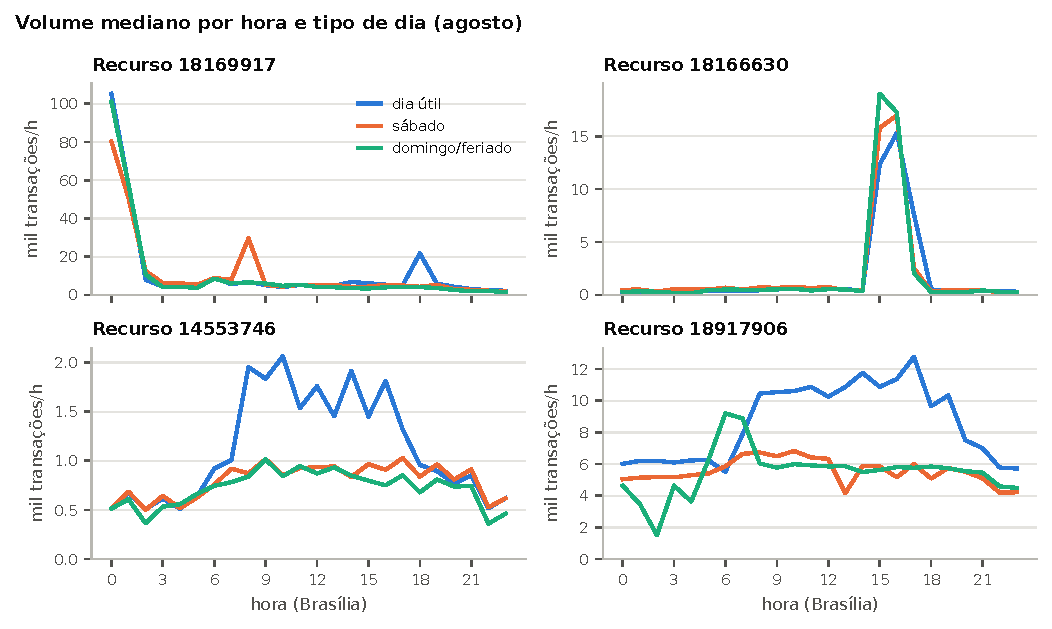
\includegraphics[width=0.92\textwidth]{figuras/fig_perfis_volume.pdf}
  \caption{Volume mediano por hora e tipo de dia em agosto, em quatro recursos representativos.}
  \label{fig:perfis}
\end{figure*}

\begin{figure*}[t]
  \centering
  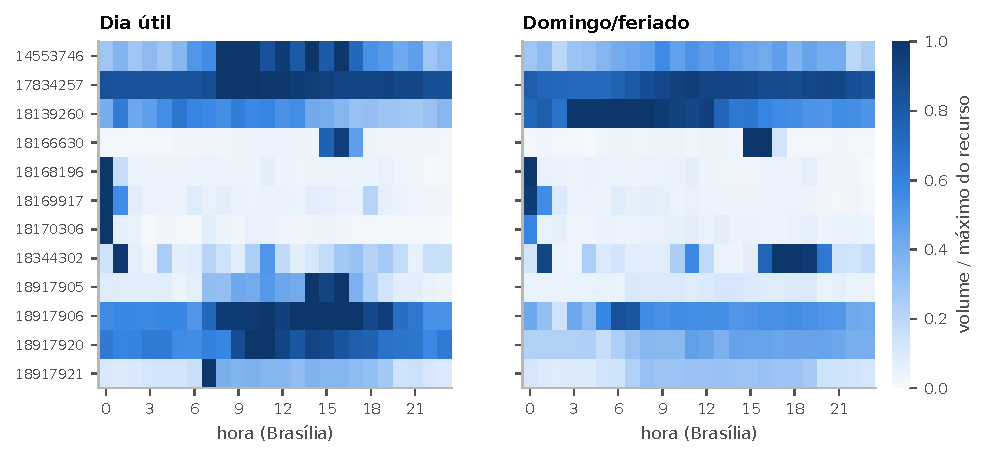
\includegraphics[width=0.85\textwidth]{figuras/fig_mapa_calor_volume.pdf}
  \caption{Volume mediano por hora, normalizado pelo máximo de cada recurso, em dias úteis e domingos/feriados.}
  \label{fig:mapa}
\end{figure*}

Nos testes de Kruskal-Wallis, 85\% das combinações recurso $\times$ atributo diferem significativamente entre as horas do dia (Holm, $\alpha=0{,}05$), com efeito grande no volume (mediana de $\varepsilon^2=0{,}39$). O volume difere entre dia útil e sábado em 6 dos 12 recursos, mas entre sábado e domingo em apenas 4. Esses quatro recursos receberam três tipos de dia; os demais, dois.

O k-means encontrou de 2 a 8 regimes por recurso (mediana 3,5), com silhouette médio de 0,46 (Tabela~\ref{tab:recursos}). Os regimes estão associados à hora (V de Cramér médio de 0,44) mais do que ao tipo de dia (0,25). Em 7 recursos os regimes foram estáveis entre as quinzenas (ARI entre 0,42 e 0,80). Nos 5 recursos com $k=2$ o ARI ficou próximo de zero: a partição ótima separa um padrão raro (por exemplo, o lote) e muda entre quinzenas. A Figura~\ref{fig:regimes} ilustra a nomeação: no recurso 14553746, o regime de volume alto ocupa as 7--17h dos dias úteis e dá lugar a um regime de volume médio no restante do tempo.

\begin{figure*}[t]
  \centering
  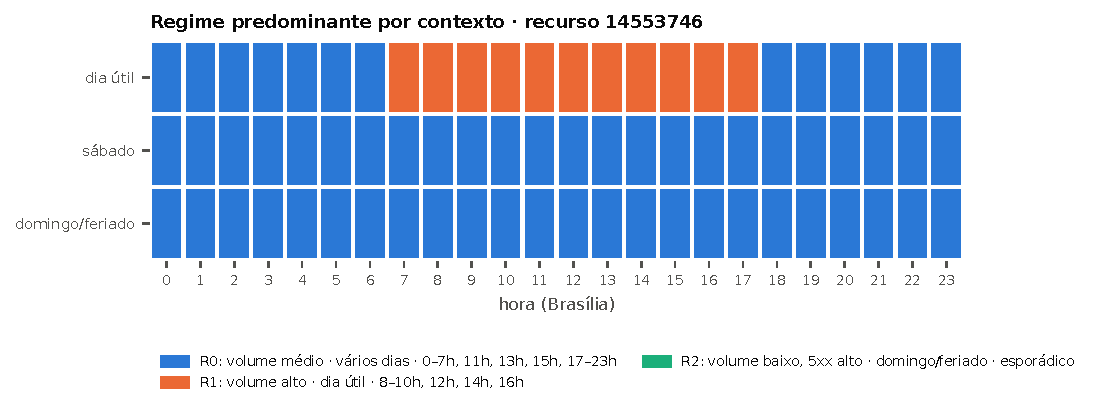
\includegraphics[width=0.85\textwidth]{figuras/fig_regimes_contexto.pdf}
  \caption{Regime predominante (k-means com atributos de comportamento) por tipo de dia e hora no recurso 14553746.}
  \label{fig:regimes}
\end{figure*}

\begin{table*}[t]
  \caption{Resumo por recurso: participação no volume, clientes, regimes (E1), tipos de dia adotados, limiar $\tau$ e recall por episódio (E2).}
  \label{tab:recursos}
  \small
  \begin{tabular}{lrrrrrrcrr}
    \toprule
    Recurso & Vol. (\%) & Clientes & $k$ & Silhouette & ARI quinzenas & V hora & Tipos de dia & $\tau_r$ & Recall ep. \\
    \midrule
    18169917 & 36,1 & 36  & 2 & 0,29 & 0,01  & 0,68 & 2 & 1,62 & 0,40 \\
    18917906 & 20,1 & 524 & 6 & 0,49 & 0,71  & 0,49 & 2 & 1,73 & 0,30 \\
    18917920 & 5,7  & 221 & 6 & 0,36 & 0,67  & 0,40 & 3 & 1,56 & 0,30 \\
    18344302 & 4,9  & 20  & 8 & 0,23 & 0,42  & 0,31 & 2 & 1,72 & 0,26 \\
    18166630 & 4,8  & 18  & 2 & 0,40 & 0,00  & 0,72 & 3 & 3,27 & 0,38 \\
    18917921 & 4,7  & 735 & 4 & 0,47 & 0,55  & 0,58 & 2 & 1,69 & 0,30 \\
    18170306 & 4,7  & 36  & 2 & 0,84 & 0,00  & 0,22 & 3 & 2,25 & 0,22 \\
    18139260 & 4,6  & 38  & 6 & 0,25 & 0,42  & 0,42 & 3 & 2,05 & 0,26 \\
    18168196 & 4,1  & 27  & 2 & 0,51 & 0,01  & 0,47 & 2 & 1,82 & 0,52 \\
    17834257 & 4,0  & 2   & 2 & 0,85 & $-$0,01 & 0,16 & 2 & 1,35 & 0,12 \\
    18917905 & 3,9  & 575 & 7 & 0,50 & 0,77  & 0,38 & 2 & 1,86 & 0,10 \\
    14553746 & 2,4  & 735 & 3 & 0,31 & 0,80  & 0,47 & 2 & 2,17 & 0,28 \\
    \bottomrule
  \end{tabular}
\end{table*}

\subsection{Perfil de normalidade e calibração}
A Figura~\ref{fig:faixa} mostra a faixa normal de volume de um recurso com lote às 15--16h: a mesma quantidade de transações é normal às 15h e residual às 10h. Os limites por atributo (Figura~\ref{fig:limites}) variam de 3 a 86 em $z$. O maior limite é o da taxa de 4xx do recurso 18344302, que em agosto teve rajadas de 4xx de um ou dois clientes repetidas à 0h e às 19h. Com esses limites, $\tau_r$ ficou entre 1,35 e 3,27 (mediana 1,78), e cerca de 1\% das janelas de agosto foram marcadas como residuais fora da amostra. Nessas janelas reais, o método encontrou 68 sequências residuais, 55 delas de uma única janela.

\begin{figure}[t]
  \centering
  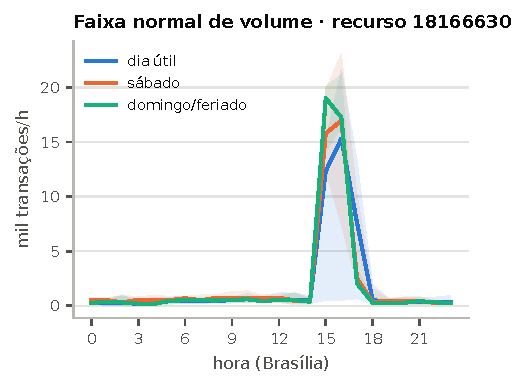
\includegraphics[width=0.9\columnwidth]{figuras/fig_faixa_normal.pdf}
  \caption{Mediana e faixa p5--p95 do volume por hora e tipo de dia (recurso 18166630).}
  \label{fig:faixa}
\end{figure}

\begin{figure}[t]
  \centering
  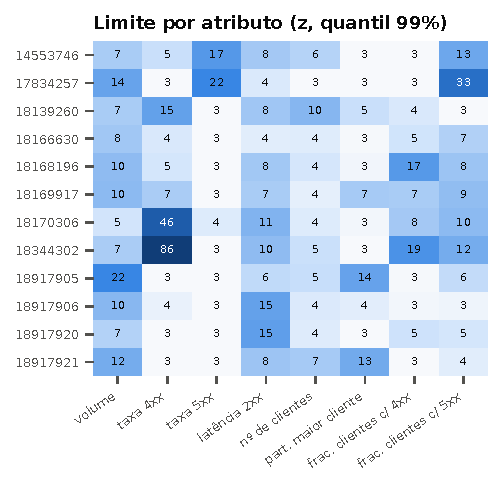
\includegraphics[width=0.9\columnwidth]{figuras/fig_limites_atributo.pdf}
  \caption{Limite de cada atributo por recurso: quantil 99\% do $z$ fora da amostra em agosto (mínimo 3).}
  \label{fig:limites}
\end{figure}

\subsection{E2: detecção Normal/Residual}
A Tabela~\ref{tab:metodos} e a Figura~\ref{fig:metodos} resumem a detecção. O perfil contextual obteve F1 por episódio de 0,41 com 0,6\% de alarmes em janelas limpas. Ele supera significativamente o percentil global (+0,08; $p=0{,}006$) e a semana anterior (+0,035; $p=0{,}04$); contra o z-score global, a diferença (+0,028) não foi significativa ($p=0{,}16$; melhor em 7 de 10 sementes). Entre as variantes, usar só a hora (0,42) equivale ao método proposto ($p=0{,}23$). Usar três tipos de dia em todos os recursos piora o resultado (0,38; $p=0{,}01$) e dobra os alarmes (1,2\%), porque os perfis de sábado e de domingo ficam com poucas amostras. Por janela, os métodos têm PR-AUC próxima (0,33 a 0,40).

\begin{table*}[t]
  \caption{E2: detecção no teste (média $\pm$ desvio-padrão em 10 sementes). $p$: Wilcoxon pareado do F1 por episódio contra o método proposto.}
  \label{tab:metodos}
  \small
  \begin{tabular}{lcccccccc}
    \toprule
    & \multicolumn{4}{c}{Por janela} & & \multicolumn{3}{c}{Por episódio} \\
    \cmidrule(lr){2-5}\cmidrule(lr){7-9}
    Método & Precisão & Recall & F1 & PR-AUC & Alarmes & Recall & Precisão & F1 ($p$) \\
    \midrule
    \textbf{Perfil contextual (proposto)} & 0,78$\pm$0,05 & 0,23$\pm$0,04 & 0,35$\pm$0,05 & 0,40$\pm$0,04 & 0,6\% & 0,30$\pm$0,05 & 0,66$\pm$0,06 & \textbf{0,41}$\pm$0,06 \\
    Perfil 3 tipos de dia & 0,66$\pm$0,06 & 0,23$\pm$0,04 & 0,34$\pm$0,05 & 0,37$\pm$0,04 & 1,2\% & 0,31$\pm$0,05 & 0,49$\pm$0,05 & 0,38 (0,010) \\
    Perfil 2 tipos de dia & 0,82$\pm$0,05 & 0,22$\pm$0,03 & 0,35$\pm$0,05 & 0,40$\pm$0,04 & 0,5\% & 0,29$\pm$0,05 & 0,68$\pm$0,07 & 0,40 (0,084) \\
    Perfil só hora & 0,81$\pm$0,04 & 0,22$\pm$0,03 & 0,35$\pm$0,04 & 0,40$\pm$0,03 & 0,5\% & 0,30$\pm$0,05 & 0,69$\pm$0,08 & 0,42 (0,232) \\
    Perfil sem feriado & 0,78$\pm$0,05 & 0,22$\pm$0,04 & 0,35$\pm$0,05 & 0,39$\pm$0,04 & 0,6\% & 0,30$\pm$0,05 & 0,66$\pm$0,06 & 0,41 (1,000) \\
    z-score global & 0,81$\pm$0,03 & 0,23$\pm$0,02 & 0,35$\pm$0,03 & 0,40$\pm$0,03 & 0,5\% & 0,27$\pm$0,04 & 0,66$\pm$0,05 & 0,38 (0,160) \\
    Percentil global p1--p99 & 0,65$\pm$0,06 & 0,21$\pm$0,03 & 0,31$\pm$0,04 & 0,33$\pm$0,03 & 1,1\% & 0,25$\pm$0,05 & 0,50$\pm$0,07 & 0,33 (0,006) \\
    Semana anterior & 0,80$\pm$0,03 & 0,23$\pm$0,02 & 0,35$\pm$0,02 & 0,40$\pm$0,03 & 0,6\% & 0,26$\pm$0,03 & 0,66$\pm$0,07 & 0,38 (0,037) \\
    \bottomrule
  \end{tabular}
\end{table*}

\begin{figure*}[t]
  \centering
  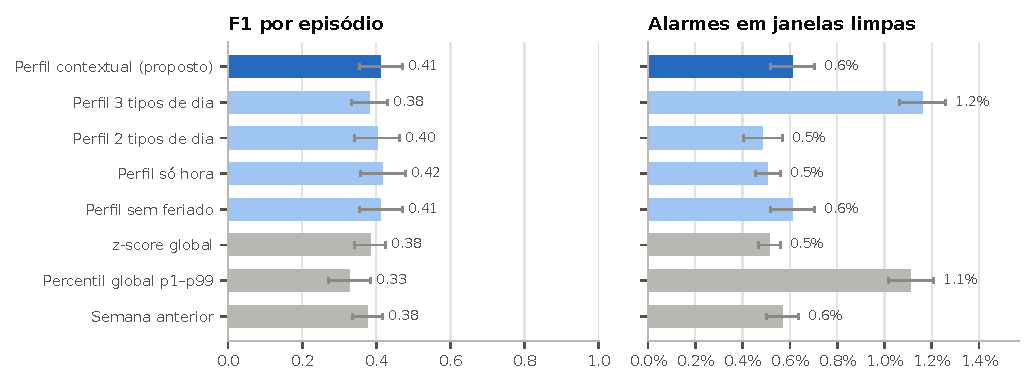
\includegraphics[width=0.9\textwidth]{figuras/fig_metodos.pdf}
  \caption{F1 por episódio e taxa de alarmes em janelas limpas por método (média e desvio-padrão em 10 sementes).}
  \label{fig:metodos}
\end{figure*}

A sensibilidade depende fortemente do tipo de falha (Figura~\ref{fig:recall}). Picos de 5xx são detectados em 71\% dos episódios (83\% na intensidade alta), 4xx concentrados em um cliente em 41\% e latência elevada em 27\% (41\% com latência $\times$4). Quedas de volume (5\%) e rajadas de um cliente (7\%) raramente são detectadas. Em relação aos baselines, o ganho do contexto aparece sobretudo nas falhas do consumidor: 4xx de um cliente (0,41 contra 0,33--0,34) e rajada (0,07 contra no máximo 0,05). A curva de operação (Figura~\ref{fig:curva}) mostra que o perfil contextual domina ou empata com os baselines em toda a faixa de alarmes; com 2\% de alarmes, o recall por episódio chega a 0,39. No feriado de 07/09, o método proposto não gerou alarmes, assim como a variante sem tratamento de feriado; a variante com três tipos de dia gerou 2,6\%.

\begin{figure}[t]
  \centering
  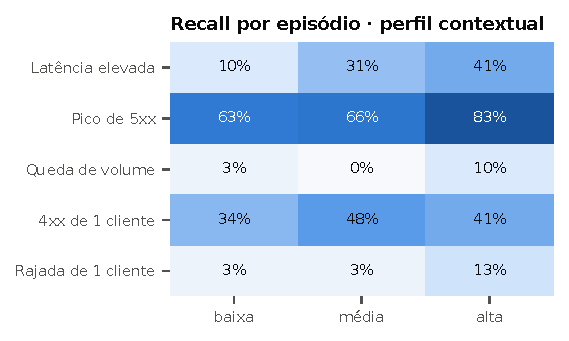
\includegraphics[width=0.85\columnwidth]{figuras/fig_recall_tipo_intensidade.pdf}
  \caption{Recall por episódio do método proposto, por tipo de falha e intensidade.}
  \label{fig:recall}
\end{figure}

\begin{figure}[t]
  \centering
  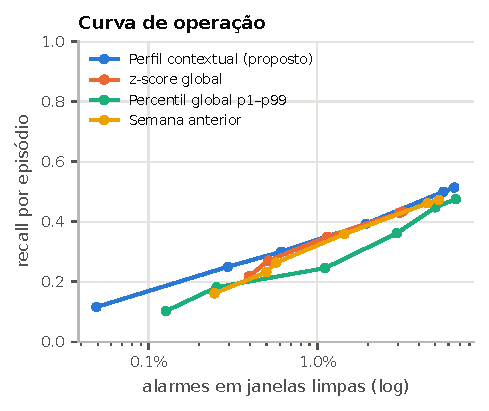
\includegraphics[width=0.85\columnwidth]{figuras/fig_curva_operacao.pdf}
  \caption{Curva de operação: recall por episódio contra alarmes em janelas limpas, variando a meta de calibração de 0,2\% a 10\%.}
  \label{fig:curva}
\end{figure}

\subsection{E3: consulta pré-incidente}
A Figura~\ref{fig:exemplo} ilustra uma consulta: um pico de 5xx de intensidade média injetado por 6~h no recurso 18169917 leva o escore normalizado de valores abaixo de 1 para cerca de 5, três vezes o limiar $\tau_r=1{,}62$. A faixa normal do contexto (em azul) acomoda o aumento de 5xx que ocorre, em dias normais, no início da madrugada.

\begin{figure*}[t]
  \centering
  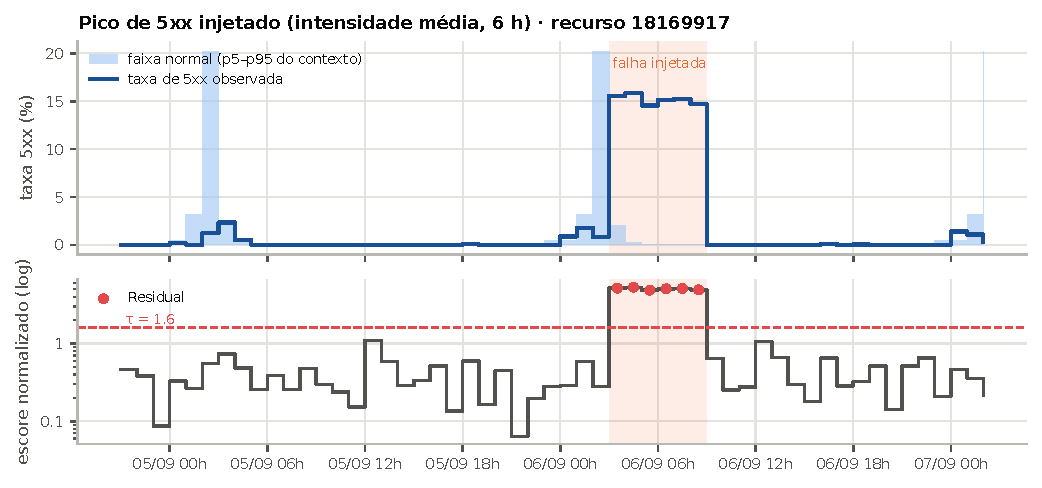
\includegraphics[width=0.9\textwidth]{figuras/fig_exemplo_episodio.pdf}
  \caption{Exemplo de episódio (semente 0): taxa de 5xx observada contra a faixa normal do contexto (acima) e escore normalizado contra o limiar $\tau_r$ (abaixo).}
  \label{fig:exemplo}
\end{figure*}

Na consulta das 6~h anteriores ao registro (Tabela~\ref{tab:consultas}), o método classificou como \Residual 27,7\% dos períodos com falha e como \Normal 98,0\% dos períodos de controle. Quando detectado, o início do desvio foi estimado com erro mediano de 0,1~h, e em 88\% dos casos com erro de até uma janela. O lado provável foi atribuído em 100\% dos períodos residuais, com 92,8\% de acerto: 88\% dos 4xx de um cliente foram atribuídos ao consumidor, e 94\% dos picos de 5xx, 100\% das latências e 100\% das quedas de volume ao provedor. As rajadas detectadas foram atribuídas ao consumidor em 75\% dos casos. O acerto do lado depende pouco do método de detecção: os baselines, avaliados com a mesma matriz, ficaram entre 91\% e 95\%.

\begin{table}[t]
  \caption{E3: consulta das 6~h anteriores ao registro (média em 10 sementes).}
  \label{tab:consultas}
  \small
  \begin{tabular}{lcccc}
    \toprule
    Método & Sensib. & Especif. & Início $\leq$1 jan. & Lado \\
    \midrule
    \textbf{Perfil contextual} & \textbf{0,28} & \textbf{0,98} & 0,88 & 0,93 \\
    z-score global & 0,27 & 0,98 & 0,88 & 0,94 \\
    Percentil global & 0,24 & 0,97 & 0,91 & 0,91 \\
    Semana anterior & 0,25 & 0,98 & 0,94 & 0,95 \\
    \bottomrule
  \end{tabular}
\end{table}

A saída da consulta é um documento estruturado. O exemplo abaixo, resumido, corresponde a um pico de 5xx de baixa intensidade injetado às 22h de 03/09. O início foi estimado exatamente e o lado foi atribuído corretamente.

\begin{Verbatim}[fontsize=\scriptsize,frame=single]
{"recurso": 18139260, "estado": "Residual",
 "periodo_analisado": {"inicio": "2026-09-03 19:00",
                       "fim": "2026-09-04 01:00"},
 "contexto": {"tipo_dia": ["dia útil"], "horas": "0h, 19–23h"},
 "residual": {"inicio_estimado": "2026-09-03 22:00",
              "duracao_janelas": 4, "persistente": true},
 "evidencias": [{"atributo": "frac. clientes c/ 5xx",
     "observado": "61.5%", "faixa_normal_p5_p95": ["0.0%","0.0%"],
     "vezes_o_limite": 6.84},
   {"atributo": "taxa 5xx", "observado": "4.6%",
     "faixa_normal_p5_p95": ["0.0%","0.0%"], "vezes_o_limite": 1.53}],
 "abrangencia": {"clientes_ativos": 13, "clientes_com_5xx": 8},
 "lado_provavel": "provedor",
 "regra": "5xx elevado e espalhado entre clientes",
 "sugestao_triagem": "Direcionar à equipe responsável pelo
   recurso 18139260 (lado provedor) ...; 8 clientes afetados."}
\end{Verbatim}

\subsection{E4: atributos relevantes}
A Figura~\ref{fig:atributos} mostra, para cada tipo de falha, a frequência com que cada atributo passou do próprio limite nas janelas residuais. Cada falha tem uma assinatura clara: pico de 5xx ativa a taxa de 5xx e a fração de clientes com 5xx (98\% e 97\%); 4xx de um cliente ativa a taxa de 4xx (97\%) e raramente a fração de clientes com 4xx (11\%), o que caracteriza a concentração; latência ativa a latência 2xx (98\%); e rajada ativa a participação do maior cliente (86\%) e o volume (71\%). Nas janelas residuais reais do teste (sem injeção), predominaram a fração de clientes com 5xx (50\%), a latência (40\%) e o volume (30\%). Entre elas, o recurso 18917906 teve, à 01h de 02/09, 5xx em 24 de 31 clientes: um candidato a incidente real.

\begin{figure*}[t]
  \centering
  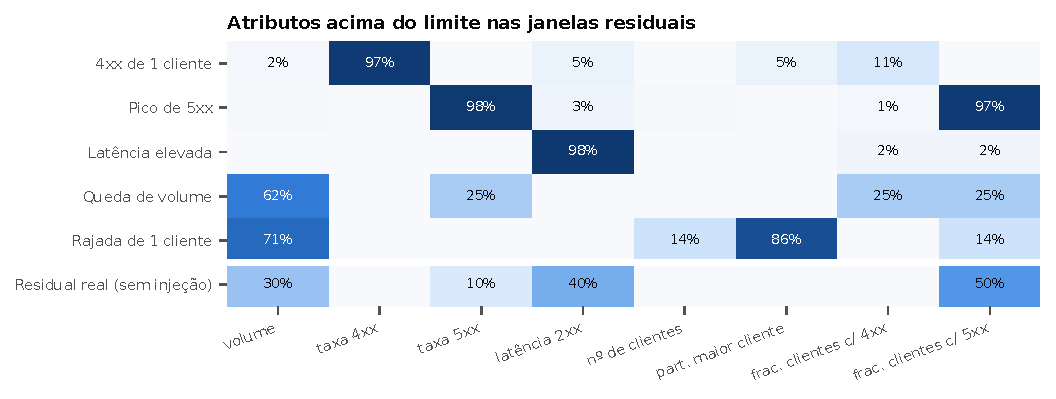
\includegraphics[width=0.9\textwidth]{figuras/fig_atributos.pdf}
  \caption{Frequência com que cada atributo passou do próprio limite nas janelas residuais, por tipo de falha (10 sementes), e nas janelas residuais reais do teste.}
  \label{fig:atributos}
\end{figure*}

\subsection{E5: tamanho da janela}
A janela de 1~h obteve o maior F1 por episódio do método proposto (Tabela~\ref{tab:janelas}). Janelas menores aumentam o recall, mas também os alarmes, e reduzem a acurácia do lado (0,79 com 15~min), porque os atributos por cliente ficam ruidosos. A janela de 4~h dilui episódios curtos: 10 dos 44 episódios por semente deixam de cobrir metade de uma janela, a sensibilidade da consulta cai para 0,08 e o erro no início sobe para 1,7~h.

\begin{table}[t]
  \caption{E5: método proposto por tamanho de janela (média em 10 sementes) e F1 do melhor baseline.}
  \label{tab:janelas}
  \small
  \begin{tabular}{lcccccc}
    \toprule
    Janela & F1 ep. & Alarmes & Sensib. & Especif. & Lado & Melhor base \\
    \midrule
    15 min & 0,35 & 0,6\% & 0,30 & 0,94 & 0,79 & 0,32 \\
    30 min & 0,38 & 0,5\% & 0,28 & 0,96 & 0,84 & 0,39 \\
    \textbf{1 h} & \textbf{0,41} & 0,6\% & 0,28 & 0,98 & 0,93 & 0,38 \\
    4 h & 0,37 & 0,8\% & 0,08 & 0,99 & 0,93 & 0,35 \\
    \bottomrule
  \end{tabular}
\end{table}

\subsection{Critérios de sucesso}
Os cinco critérios definidos no entendimento do negócio foram atendidos (Tabela~\ref{tab:criterios}). O primeiro deve ser lido com cautela: a vantagem sobre o z-score global não foi estatisticamente significativa.

\begin{table}[t]
  \caption{Critérios de sucesso definidos antes da modelagem.}
  \label{tab:criterios}
  \small
  \begin{tabular}{p{0.5\columnwidth}p{0.22\columnwidth}c}
    \toprule
    Critério & Resultado & Atendido \\
    \midrule
    F1 por episódio $>$ melhor baseline & 0,41 vs 0,38 & sim$^\ast$ \\
    Alarmes em janelas limpas $\leq$ 2\% & 0,61\% & sim \\
    Erro mediano no início $\leq$ 1 janela & 0,1 h & sim \\
    Acurácia do lado provável $\geq$ 70\% & 92,8\% & sim \\
    Controles com saída Normal $\geq$ 95\% & 98,0\% & sim \\
    \bottomrule
  \end{tabular}
  \par\smallskip\footnotesize $^\ast$Diferença não significativa contra o z-score global ($p=0{,}16$).
\end{table}

%% =====================================================================
\section{Discussão}\label{sec:discussao}

\paragraph{RQ1: regimes e separação Normal/Residual.} Os AALs agregados mostram regimes claros e ligados ao contexto em todos os recursos, sobretudo à hora do dia: lotes na virada do dia e à tarde, padrão comercial em dias úteis e comportamento mais plano no fim de semana. A caracterização por k-means é útil para descrever e nomear esses regimes, mas instável nos recursos dominados por um único padrão raro; por isso, a decisão \Normal/\Residual usa o perfil por contexto, e não os grupos. Na detecção, o contexto trouxe ganho consistente sobre o percentil global e a semana anterior, e ganho pequeno e não significativo sobre um z-score global bem calibrado. O efeito do contexto vem quase todo da hora; separar sábado de domingo em todos os recursos piorou o resultado. Isso indica que, com um mês de treino, a parcimônia no contexto importa tanto quanto sua riqueza. A decisão adaptativa por recurso, tomada só com dados de agosto, evitou essa perda.

\paragraph{O limite por atributo.} A principal decisão de modelagem foi normalizar cada atributo pela sua própria cauda no recurso. Sem isso, os atributos com picos reais frequentes (taxas de 4xx) definem o limiar e escondem desvios de latência e volume. Esse achado é, por si, relevante para a prática: em AALs reais, os atributos não têm a mesma variabilidade, e um único limiar global sobre todos eles tende a privilegiar os mais ruidosos.

\paragraph{RQ2: utilidade para a triagem.} Quando o desvio é detectado, a informação produzida é precisa: o início é estimado quase sempre na janela correta, e o lado provável acerta 93\% dos casos. Um período classificado como \Normal também é informativo: com 98\% de especificidade, ele indica ao operador que o recurso dificilmente é a origem do incidente. A limitação é a sensibilidade: apenas 28\% dos períodos com falha são sinalizados. Na prática, isso significa que um resultado \Residual é forte evidência, mas um resultado \Normal não descarta falhas sutis, sobretudo de volume.

\paragraph{RQ3: atributos relevantes.} As taxas de erro e as frações de clientes com erro são os atributos mais discriminantes, e a combinação ``taxa alta'' com ``fração de clientes alta ou baixa'' é o que separa provedor de consumidor. A latência é o segundo sinal mais útil. O volume é o atributo menos sensível, porque sua variação dentro de um mesmo contexto já é grande.

\paragraph{Por que o volume é pouco sensível.} Uma queda de 50\% do volume equivale a $\log 2\approx0{,}69$ na escala logarítmica. A escala robusta mediana do volume nos contextos é 0,38 (quartis 0,22 e 0,61), de modo que essa queda produz $z\approx1{,}8$, enquanto o limite do volume (Figura~\ref{fig:limites}) fica entre 5 e 22. Assim, só quedas muito fortes ultrapassam o limite. Atributos que controlem a variação do volume (por exemplo, a razão entre o volume do recurso e o volume total do gateway) são um caminho natural de melhoria.

%% =====================================================================
\section{Ameaças à validade}\label{sec:ameacas}

\paragraph{Falhas sintéticas.} O desempenho mede a capacidade de detectar \emph{os tipos injetados}, e não falhas reais. As intensidades variadas, as 10 sementes e a comparação com baselines reduzem, mas não eliminam, esse viés. A matriz de lado e o gerador de falhas foram concebidos pelo mesmo autor, o que pode favorecer a acurácia do lado. Essa acurácia também é medida apenas sobre episódios detectados, que tendem a ser os mais fortes.

\paragraph{Treino curto.} Um mês de dados resulta em cerca de 5 amostras por hora para cada tipo de dia não útil, o que torna as faixas de fim de semana largas e explica a piora com três tipos de dia. Não foi possível avaliar sazonalidades mensais (fechamento de mês, por exemplo).

\paragraph{Decisões durante a execução.} Duas decisões foram tomadas após observar dados de treino: a calibração por validação cruzada (em vez de uma única semana) e o limite por atributo. Ambas usaram apenas dados de agosto; a semana de teste não participou de nenhuma escolha. A escolha do tamanho da janela (E5), porém, usa o teste e deve ser vista como exploratória.

\paragraph{Anomalias reais não rotuladas.} Janelas limpas do teste podem conter anomalias reais (como a do recurso 18917906), contadas como falso alarme. A taxa de alarmes é, portanto, uma estimativa conservadora.

\paragraph{Generalização.} Os resultados vêm de uma organização e de 12 recursos, sendo um com apenas dois clientes (lado indeterminado para regras de abrangência) e quatro com dados de teste encerrados em 03/09. A base não pode ser compartilhada, o que limita a reprodutibilidade externa; o código dos notebooks, porém, é independente dos dados.

%% =====================================================================
\section{Considerações finais}\label{sec:conclusao}

Este trabalho mostrou que Access Logs agregados, sem \emph{traces} nem logs de aplicação, permitem caracterizar os regimes normais de cada recurso de API e produzir, para um incidente registrado, uma informação explicável sobre o período anterior: estado \Normal ou \Residual, início do desvio, evidências com a faixa normal do contexto, abrangência entre clientes e lado provável. O método é simples (mediana, MAD, quantis e uma matriz heurística), não exige rótulos e cabe na rotina de uma equipe de operação.

Os resultados indicam que a informação é confiável quando emitida (93\% de acerto no lado provável, início quase sempre na janela correta, 98\% de especificidade), mas que a sensibilidade ainda é limitada (28--30\%), especialmente para desvios de volume. O contexto horário é o que mais contribui; o ganho sobre um z-score global bem calibrado é pequeno.

Como trabalhos futuros, destacam-se: (i) validar o método com incidentes reais e com a avaliação qualitativa de operadores; (ii) usar um histórico mais longo, para capturar sazonalidades mensais e tornar viáveis perfis de fim de semana; (iii) incorporar atributos relativos ao volume do gateway, para melhorar a sensibilidade a desvios de volume; (iv) avaliar a generalização para outras APIs; e (v) integrar a consulta como ferramenta de um agente de triagem e medir seu efeito no direcionamento dos incidentes.

\bibliographystyle{ACM-Reference-Format}
\bibliography{referencias}

\end{document}
